\documentclass{article}
\usepackage{CJK}
\usepackage{amsmath,amssymb,graphicx,mathrsfs}

%%%%%%%%%% Start TeXmacs macros
\newcommand{\nobracket}{}
\newcommand{\tmaffiliation}[1]{\\ #1}
\newcommand{\tmmathbf}[1]{\ensuremath{\boldsymbol{#1}}}
\newcommand{\tmop}[1]{\ensuremath{\operatorname{#1}}}
%%%%%%%%%% End TeXmacs macros

\begin{document}
\begin{CJK*}{UTF8}{gbsn}

\title{FDFD Tutorial from zero}

\author{
  Zhijun Zeng
  \tmaffiliation{2023年10月15日}
}

\maketitle

\

\

\section{简介}

在需要瞬态解或者宽带分析时,FDFD非常有用。
\begin{enumerate}
  \item 比如我们感兴趣单一频率上的稳态解,FDFD
  不需要时间上步进,只用求解单个矩阵逆。
  
  \item
  对于色散材料,我们可以简单的使用标量或者向量建模,在FDTD中需要卷积或者辅助方程。
\end{enumerate}

\section{电磁学理论}

\subsection{Maxwell's Equations}

麦克斯韦方程组由库仑定律,安培定律,法拉第定律,电荷守恒组成。
\begin{enumerate}
  \item 法拉第定律:磁通量的变化会产生电动势
  \[ \oint_C \bar{E} \cdot d\tmmathbf{l}= - \int_S \frac{\partial
     \bar{B}}{\partial t} \cdot d\tmmathbf{s}, \nabla \times \bar{E} =
     \frac{\partial \bar{B}}{\partial t} \]
  其中$\bar{E}$为感生电场,$\bar{B}$为磁感应强度。
  
  \item 高斯定律:闭合曲面内电荷分布与磁场关系
  \[ \oint_S \bar{D} \cdot d\tmmathbf{s}= \int_V \bar{\rho} \tmop{dv}, \nabla
     \cdot \bar{D} = \bar{\rho} \]
  其中$\bar{D}$为电位移矢量,与电场强度成正比。
  
  \item
  安培定律:磁场对闭合曲线的线积分等于内部的总电流
  \[ \oint_C \bar{H} \cdot d\tmmathbf{l}= \int_S \bar{J} \cdot d\tmmathbf{s}+
     \int_S \frac{\partial \bar{D}}{\partial t} \cdot d\tmmathbf{s}, \nabla
     \times \bar{H} = \bar{J} + \frac{\partial \bar{D}}{\partial t} \]
  其中$\bar{H}$为磁场强度,与磁感应强度成正比,$\bar{J}$为电流密度
  
  \item 磁感线闭合:
  \[ \oint_S \bar{B} \cdot d\tmmathbf{s}= 0, \nabla \cdot \bar{B} = 0 \]
\end{enumerate}
结合3与2可以得到连续性方程
\[ - \oint_S \bar{J} \cdot d\tmmathbf{s}= \frac{\partial}{\partial t} \int_V
   \bar{\rho} \tmop{dv}, \nabla \cdot \bar{J} = - \frac{\partial
   \bar{\rho}}{\partial t} \]
这里我们用到了stokes 定理和散度定理
\begin{enumerate}
  \item Stokes:
  \[ \oint_C G \cdot d\tmmathbf{l}= \int_S \nabla \times G \cdot d\tmmathbf{s}
  \]
  \item Divergence:
  \[ \oint_S G \cdot d\tmmathbf{s}= \int_V \nabla \cdot \tmop{Gdv} \]
\end{enumerate}


\subsection{Constitutive relations and material properties}

在简单情形下,电场强度与电通量密度相差常数,磁场强度与磁通量密度也相差常数,
\[ \bar{D} = \tilde{\varepsilon} \bar{E}, \bar{B} = \tilde{\mu} \bar{H} \]
电流密度$\bar{J} = \bar{J}_i +
\overline{J_c},$其中i项为外部施加的源电流,c项$\overline{E_c} =
\tilde{\sigma} \bar{E}$为传导电流,通过导电介质传导。

\

在一般情形下,介质是inhomogeneus的
\[ \bar{D} (\tmmathbf{r}, t) = \tilde{\varepsilon} (\tmmathbf{r}, t) \bar{E}
   (\tmmathbf{r}, t), \bar{B} (\tmmathbf{r}, t) = \tilde{\mu} (\tmmathbf{r},
   t) \bar{H} (\tmmathbf{r}, t), \bar{J} (\tmmathbf{r}, t) = \tilde{\sigma}
   (\tmmathbf{r}, t) \bar{E} (\tmmathbf{r}, t) \]
对于色散介值,$\varepsilon (\omega) = \varepsilon_0 [1 + \chi_e
(\omega)]$,在频域空间。

\subsection{Time-harmonic Maxwell's equations}

Time harmonic 的Maxwell's
equations在很多场景(广播,雷达,光学,微波应用)中存在,此时发射源为窄频段,导致所有场的分量的行为与中心单频正弦相似,电场和磁场随着时间呈正弦变化,此时瞬态解并不重要,人们更关心稳态的正弦近似。

Time harmonic(sinusoidal steady state ) form :
\[ \begin{array}{c}
     \nabla \times \bar{E} = \frac{\partial \bar{B}}{\partial t} \Rightarrow
     \nabla \times \tmmathbf{E}= - j \omega \tmmathbf{B}\\
     \nabla \cdot \bar{D} = \bar{\rho} \Rightarrow \nabla \cdot \tmmathbf{D}=
     \rho\\
     \nabla \times \bar{H} = \bar{J} + \frac{\partial \bar{D}}{\partial t}
     \Rightarrow \nabla \times \tmmathbf{H}=\tmmathbf{J}+ j \omega
     \tmmathbf{D}\\
     \nabla \cdot \bar{B} = 0 \Rightarrow \nabla \cdot \tmmathbf{B}= 0
   \end{array} \]
在上面方程中,场变量$\bar{E}, \bar{D}, \bar{H},
\bar{B}$是实的随时间变化的量,而向量$\tmmathbf{E}, \tmmathbf{B},
\tmmathbf{H}, \tmmathbf{D}$为复的,不随时间变化的量。

他们之间通过如下转化
\[ E (x, y, z, y) = \tmop{Re} \{ \tmmathbf{E} (x, y, z) e^{j \omega t} \} \]
对于一些量也是这样
\[ \bar{\rho} (x, y, z, t) = \tmop{Re} \{ \rho (x, y, z) e^{j \omega t} \} \]
对于dispersive materials, $\varepsilon, \mu,
\sigma$为随频率改变的,我们有
\[ \tmmathbf{D} (\omega) = \varepsilon (\omega) \tmmathbf{E} (\omega),
   \tmmathbf{B} (\omega) = \mu (\omega) \tmmathbf{H} (\omega), \tmmathbf{J}
   (\omega) = \sigma (\omega) \tmmathbf{E} (\omega) \]

\subsection{边界条件}

边界条件描述了材料之间的界面上的电磁波相互作用。
\begin{enumerate}
  \item 切向电场在交界面处连续,
  由将第一方程作用在交界面处得到
  \[ \tmmathbf{n} \times [\overline{E_1} - \bar{E}_2] = 0 \rightarrow E_{1 t}
     = E_{2 t} \]
  \item
  切向磁场在交界面处连续,由将第三方程作用在交界面处得到
  \[ \tmmathbf{n} \times [\overline{H_1} - \bar{H}_2] = 0 \rightarrow H_{1 t}
     = H_{2 t} \]
  除非存在表面电流,此时$\tmmathbf{n} \times \bar{H}_1 =
  \bar{J}_s$, 此时$\bar{H}_2 = 0$对于完美导体
  
  \item
  电通量密度的法向量是连续的,除非存在表面电荷$\tilde{\rho}_s$,
  由第二方程得到
  \[ \tmmathbf{n} \cdot [\bar{D}_1 - \bar{D}_2] = \tilde{\rho}_s \rightarrow
     D_{1 n} - D_{2 n} = \widetilde{\rho_s} \]
  \item 磁感应强度法向连续,通过第四式得到
  \[ \tmmathbf{n} \cdot [\bar{B}_1 - \overline{B_2}] = 0 \rightarrow B_{1 n} =
     B_{2 n} \]
  \item 基于连续性方程可以得到
  \[ \tmmathbf{n} \cdot [\overline{J_1} - \bar{J}_2] = - \frac{\partial
     \bar{\rho}_s}{\partial t} \rightarrow J_{1 n} - J_{2 n} = -
     \frac{\partial \overline{\rho_s}}{\partial t} \]
  
\end{enumerate}

\subsection{电磁波}

虽然在FDTD中我们大部分时间在处理Maxwell's
equation的离散形式,但是我们仍然需要波方程的概念。

考虑在真空中的Maxwell's equation ,$\bar{\rho} = \bar{J} =
0$,此时$\varepsilon, \mu$与时间无关
\[ \nabla \times \bar{E} = - \mu \frac{\partial \bar{H}}{\partial t}, \nabla
   \times \bar{H} = \varepsilon \frac{\partial \bar{E}}{\partial t} \]
对第一个方程取curl,代入第二个方程
\[ \nabla \times \nabla \times \bar{E} = - \mu \frac{\partial}{\partial t}
   \nabla \times \bar{H} = - \mu \varepsilon \frac{\partial^2
   \bar{E}}{\partial^2 t} \]
而由于
\[ \nabla \times \nabla \times A = \nabla (\nabla \cdot A) - \nabla^2 A \]
由于$\bar{\rho} = 0, \nabla \cdot \bar{E} = 0$
\[ \nabla^2 \bar{E} - \mu \varepsilon \frac{\partial^2 \bar{E}}{\partial t^2}
   = 0 \]

\subsubsection{一维情形}

在一维情形下,$\bar{E} = E_x$, 一般解为
\[ E_x (z, t) = f (z - v_p t) + g (z + v_p t), v_p = \frac{1}{\sqrt{\mu
   \varepsilon}} \]
一维时谐方程为
\[ \frac{\partial^2 E_x}{\partial z^2} + k^2 E_x = 0, k^2 = \omega^2 \mu
   \varepsilon \]
解的一般形式为
\[ E_x (z, t) = \tmop{Re} \{ (C_1 e^{- \tmop{jkz}} + C_2 e^{\tmop{jkz}}) e^{j
   \omega t} \} \]
其中$k = \frac{2 \pi}{\lambda}, \omega = 2 \pi
f$为波数与角频率。相速度为$v_p = \frac{\tmop{dz}}{\tmop{dt}} =
\frac{\omega}{k}$, 群速度为$v_g = \frac{\tmop{dz}}{\tmop{dt}} =
\frac{\Delta \omega}{\Delta k}$

相速度是波前传播通过介质的速度,群速度是能量传播通过介质的速度。

\

\section{FDTD grid and Yee Algorithm}

本节内容中我们将注意力集中在FDTD算法或者Yee算法中,用于时域的Maxwell方程组求解。简单来说,在这个算法中,空间和时间的连续导数利用中心差分二阶近似得到,利用一个交错的空间网格放置电场和磁场,在时间上用蛙跳格式来更新场。

中心差分是指一个场的方向导数(如z方向)在时间$n \Delta
t,$空间点$(i, j, k)$上由
\[ \left. \frac{\partial \mathscr{G}}{\partial z} \right|_{i, j, k}^n =
   \frac{\mathscr{C}_{i, j, k + 1 / 2}^n - \mathscr{G}_{i, j, k - 1 /
   2}^n}{\Delta z} + O [(\Delta z)^2] . \]
得到,者表明需要场变量在$\left( i, j, k \pm \frac{1}{2}
\right)$处定义。

\raisebox{0.0\height}{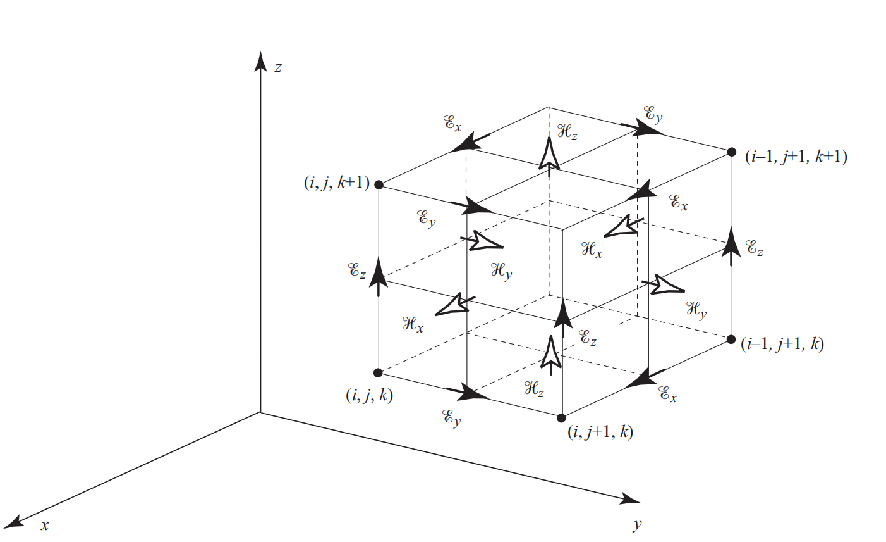
\includegraphics[width=14.874163715072806cm,height=9.102731864095501cm]{FDFD_tutorial-1.pdf}}

\

接下来的内容中我们考虑在笛卡尔系下无源,简单介质中的Maxwell方程
\[ \begin{aligned}
     \frac{\partial \mathscr{E}_x}{\partial t} & = \frac{1}{\epsilon}  \left(
     \frac{\partial \mathscr{H}_z}{\partial y} - \frac{\partial
     \mathscr{H}_y}{\partial z} \right) & \frac{\partial
     \mathscr{H}_x}{\partial t} & = \frac{1}{\mu}  \left( \frac{\partial
     \mathscr{E}_y}{\partial z} - \frac{\partial \mathscr{E}_z}{\partial y}
     \right)\\
     \frac{\partial \mathscr{E}_y}{\partial t} & = \frac{1}{\epsilon}  \left(
     \frac{\partial \mathscr{H}_x}{\partial z} - \frac{\partial
     \mathscr{H}_z}{\partial x} \right) & \frac{\partial
     \mathscr{H}_y}{\partial t} & = \frac{1}{\mu}  \left( \frac{\partial
     \mathscr{E}_z}{\partial x} - \frac{\partial \mathscr{E}_x}{\partial z}
     \right)\\
     \frac{\partial \mathscr{E}_z}{\partial t} & = \frac{1}{\epsilon}  \left(
     \frac{\partial \mathscr{H}_y}{\partial x} - \frac{\partial
     \mathscr{H}_x}{\partial y} \right) & \frac{\partial
     \mathscr{H}_z}{\partial t} & = \frac{1}{\mu}  \left( \frac{\partial
     \mathscr{E}_x}{\partial y} - \frac{\partial \mathscr{E}_y}{\partial x}
     \right) .
   \end{aligned} \]

\subsection{1D Maxwell's equation}

1D表示我们考虑去掉系统中y,z方向的导数,并不考虑磁电损失$(\sigma
= \sigma_m = 0)$,考虑简单的无源介质$\bar{\rho} = 0, \bar{J} = 0$,
$\varepsilon,
\mu$为常数,与位置无关,与方向无关,与时间无关。
\[ \begin{aligned}
     \frac{\partial \mathscr{E}_x}{\partial t} & = 0 & \frac{\partial
     \mathscr{H}_x}{\partial t} & = 0\\
     \frac{\partial \mathscr{E}_y}{\partial t} & = - \frac{1}{\epsilon} 
     \frac{\partial \mathscr{H}_z}{\partial x} & \frac{\partial
     \mathscr{H}_y}{\partial t} & = \frac{1}{\mu}  \frac{\partial
     \mathscr{E}_z}{\partial x}\\
     \frac{\partial \mathscr{E}_z}{\partial t} & = \frac{1}{\epsilon} 
     \frac{\partial \mathscr{H}_y}{\partial x} & \frac{\partial
     \mathscr{H}_z}{\partial t} & = - \frac{1}{\mu}  \frac{\partial
     \mathscr{E}_y}{\partial x} .
   \end{aligned} \]
此时电磁场的x分量不随时间改变,为常量。场变量只跟一个空间坐标x相关,故为1D。于是方程余下形式为
\begin{enumerate}
  \item 1D TM:
  \[ \begin{aligned}
       \frac{\partial \mathscr{H}_y}{\partial t} & = \frac{1}{\mu} 
       \frac{\partial \mathscr{E}_z}{\partial x}\\
       \frac{\partial \mathscr{E}_z}{\partial t} & = \frac{1}{\epsilon} 
       \frac{\partial \mathscr{H}_y}{\partial x}
     \end{aligned} \]
  \item 1D TE:
  \[ \begin{aligned}
       \frac{\partial \mathscr{E}_y}{\partial t} & = - \frac{1}{\epsilon} 
       \frac{\partial \mathscr{H}_z}{\partial x}\\
       \frac{\partial \mathscr{H}_z}{\partial t} & = - \frac{1}{\mu} 
       \frac{\partial \mathscr{E}_y}{\partial x} .
     \end{aligned} \]
  
\end{enumerate}
TM mode为磁场垂直传播方向,电场沿传播方向的电磁波,TE
mode 为电场垂直传播方向,磁场沿着传播方向的电磁波。

计算格式:
\begin{enumerate}
  \item 1D TE mode:
  \[ \begin{array}{c}
       \nobracket \mathscr{E}_y |_i^{n + 1} = \nobracket \mathscr{E}_y |_i^n -
       \frac{\Delta t}{\epsilon_i \Delta x}  [\nobracket \mathscr{H}_z |_{i +
       1 / 2}^{n + 1 / 2} - \nobracket \mathscr{H}_z |_{i - 1 / 2}^{n + 1 /
       2}]\\
       \nobracket \mathscr{H}_z |_{i + 1 / 2}^{n + 1 / 2} = \nobracket
       \mathscr{H}_z |_{i + 1 / 2}^{n - 1 / 2} - \frac{\Delta t}{\mu_{i + 1 /
       2} \Delta x}  [\nobracket \mathscr{E}_y |_{i + 1}^n - \nobracket
       \mathscr{E}_y |_i^n]
     \end{array} \]
  \item 1D TM mode:
  \[ \begin{array}{c}
       \nobracket \mathscr{H}_y |_{i + 1 / 2}^{n + 1 / 2} = \nobracket
       \mathscr{H}_y |_{i + 1 / 2}^{n - 1 / 2} + \frac{\Delta t}{\mu_{i + 1 /
       2} \Delta x}  [\nobracket \mathscr{E}_z |_{i + 1}^n - \nobracket
       \mathscr{E}_z |_i^n]\\
       \nobracket \mathscr{E}_z |_i^{n + 1} = \nobracket \mathscr{E}_z |_i^n +
       \frac{\Delta t}{\epsilon_i \Delta x}  [\nobracket \mathscr{H}_y |_{i +
       1 / 2}^{n + 1 / 2} - \nobracket \mathscr{H}_y |_{i - 1 / 2}^{n + 1 /
       2}]
     \end{array} \]
\end{enumerate}
这里需要$\mathscr{E}_y, \mathscr{E}_z$ 在n,i网格上,$\mathscr{H}_y,
\mathscr{H}_z$在$n \pm \frac{1}{2}, i \pm \frac{1}{2}$网格上.

对于初始条件,我们需要给出$\mathscr{E}_z^0,
\mathscr{H}_y^{\frac{1}{2}}$,
大家一般直接估计了$\mathscr{H}_y^{\frac{1}{2}}$,
利用一些高阶方法。

\subsection{2D Maxwell's equation}

假设不考虑z方向的导数,其他假设同1D情况,方程变为
\[ \begin{aligned}
     \frac{\partial \mathscr{H}_x}{\partial t} & = - \frac{1}{\mu} 
     \frac{\partial \mathscr{E}_z}{\partial y}\\
     - \mu \frac{\partial \overline{\mathscr{H}}}{\partial t} = \nabla \times
     \overline{\mathscr{E}} \quad \rightarrow \quad \frac{\partial
     \mathcal{H}_y}{\partial t} & = \frac{1}{\mu}  \frac{\partial
     \mathscr{E}_z}{\partial x}\\
     \frac{\partial \mathscr{H}_z}{\partial t} & = \frac{1}{\mu}  \left(
     \frac{\partial \mathscr{E}_x}{\partial y} - \frac{\partial
     \mathscr{E}_y}{\partial x} \right)
   \end{aligned} \]
\[ \
   
   \begin{aligned}
     \frac{\partial \mathscr{E}_x}{\partial t} & = \frac{1}{\epsilon} 
     \frac{\partial \mathscr{H}_z}{\partial y}\\
     \epsilon \frac{\partial \mathscr{E}}{\partial t} = \nabla \times
     \overline{\mathscr{H}} \rightarrow \frac{\partial \mathscr{E}_y}{\partial
     t} & = - \frac{1}{\epsilon}  \frac{\partial \mathscr{H}_z}{\partial x}\\
     \frac{\partial \mathscr{E}_z}{\partial t} & = \frac{1}{\epsilon}  \left(
     \frac{\partial \mathscr{H}_y}{\partial x} - \frac{\partial
     \mathscr{H}_x}{\partial y} \right) .
   \end{aligned} \]
此时场变量只跟x,y两个变量相关,故为2D。我们重组这两个式子,可以为TM
mode 和TE mode
\begin{enumerate}
  \item TM mode:
  \[ \begin{array}{ll}
       \frac{\partial \mathscr{H}_x}{\partial t} & = - \frac{1}{\mu} 
       \frac{\partial \mathscr{E}_z}{\partial y}\\
       \quad \frac{\partial \mathcal{H}_y}{\partial t} & = \frac{1}{\mu} 
       \frac{\partial \mathscr{E}_z}{\partial x}\\
       \frac{\partial \mathscr{E}_z}{\partial t} & = \frac{1}{\epsilon} 
       \left( \frac{\partial \mathscr{H}_y}{\partial x} - \frac{\partial
       \mathscr{H}_x}{\partial y} \right) .
     \end{array} \]
  \item TE mode:
  \[ \begin{array}{ll}
       \frac{\partial \mathscr{E}_x}{\partial t} & = \frac{1}{\epsilon} 
       \frac{\partial \mathscr{H}_z}{\partial y}\\
       \frac{\partial \mathscr{E}_y}{\partial t} & = - \frac{1}{\epsilon} 
       \frac{\partial \mathscr{H}_z}{\partial x}\\
       \frac{\partial \mathscr{H}_z}{\partial t} & = \frac{1}{\mu}  \left(
       \frac{\partial \mathscr{E}_x}{\partial y} - \frac{\partial
       \mathscr{E}_y}{\partial x} \right)
     \end{array} \]
\end{enumerate}
此时z方向为波的传播方向,TMmode中磁场垂直传播方向(x,y)。

\raisebox{0.0\height}{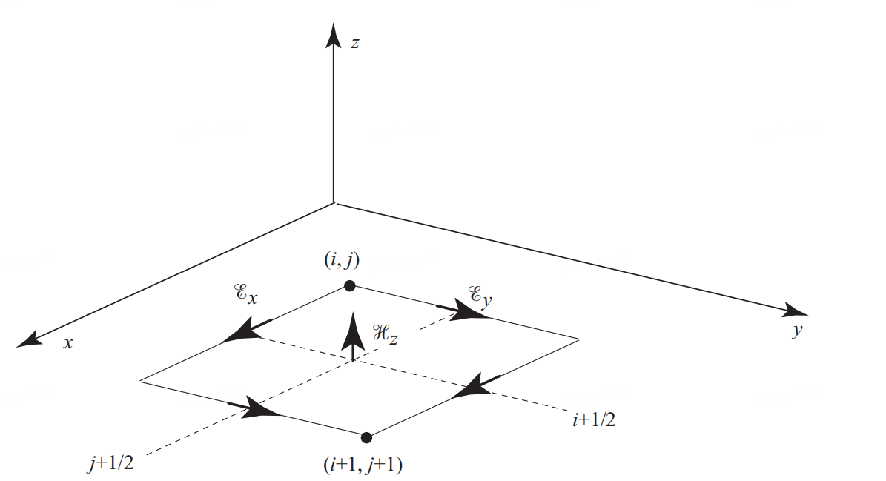
\includegraphics[width=14.874163715072806cm,height=8.07239603830513cm]{FDFD_tutorial-2.pdf}}

\subsubsection{TE mode}

在 Yee cell中,我们将$\mathscr{E}_x, \mathscr{E}_y$分别放在$\left( i
+ \frac{1}{2}, j \right), \left( i, j + \frac{1}{2}
\right)$网格中,$\mathscr{H}_z$放在$\left( i + \frac{1}{2}, j +
\frac{1}{2} \right)$中, 半离散格式为
\[ \begin{aligned}
     \left. \frac{\partial \mathscr{E}_x}{\partial t} \right|_{i + 1 / 2, j} &
     = \frac{1}{\epsilon} \left[ \frac{\nobracket \mathscr{H}_z |_{i + 1 / 2,
     j + 1 / 2} - \nobracket \mathscr{H}_z |_{i + 1 / 2, j - 1 / 2}}{\Delta y}
     \right]\\
     \left. \frac{\partial \mathscr{E}_y}{\partial t} \right|_{i, j + 1 / 2} &
     = - \frac{1}{\epsilon} \left[ \frac{\nobracket \mathscr{H}_z |_{i + 1 /
     2, j + 1 / 2} - \nobracket \mathscr{H}_z |_{i - 1 / 2, j + 1 / 2}}{\Delta
     x} \right]\\
     \left. \frac{\partial \mathscr{H}_z}{\partial t} \right|_{i + 1 / 2, j +
     1 / 2} & = \frac{1}{\mu}  \left[ \frac{\nobracket \mathscr{E}_x |_{i + 1
     / 2, j + 1} - \nobracket \mathscr{E}_x |_{i + 1 / 2, j}}{\Delta y} -
     \frac{\nobracket \mathscr{E}_y |_{i + 1, j + 1 / 2} - \nobracket
     \mathscr{E}_y |_{i, j + 1 / 2}}{\Delta x} \right]
   \end{aligned} \]
对于时间网格,与刚刚相似,得到全离散格式为
\[ \begin{array}{l}
     \nobracket \mathscr{H}_z |_{i + 1 / 2, j + 1 / 2}^{n + 1 / 2} =
     \nobracket \mathscr{H}_z |_{i + 1 / 2, j + 1 / 2}^{n - 1 / 2} +
     \frac{\Delta t}{\mu_{i + 1 / 2, j + 1 / 2}}\\
     \times \left[ \frac{\nobracket \mathscr{E}_x |_{i + 1 / 2, j + 1}^n -
     \nobracket \mathscr{E}_x |_{i + 1 / 2, j}^n}{\Delta y} - \frac{\nobracket
     \mathscr{E}_y |_{i + 1, j + 1 / 2}^n - \nobracket \mathscr{E}_y |_{i, j +
     1 / 2}^n}{\Delta x} \right]\\
     \nobracket \mathscr{E}_x |_{i + 1 / 2, j}^{n + 1} = \nobracket
     \mathscr{E}_x |_{i + 1 / 2, j}^n + \frac{\Delta t}{\epsilon_{i + 1 / 2,
     j} \Delta y}  [\nobracket \mathscr{H}_z |_{i + 1 / 2, j + 1 / 2}^{n + 1 /
     2} - \nobracket \mathscr{H}_z |_{i + 1 / 2, j - 1 / 2}^{n + 1 / 2}]\\
     \nobracket \mathscr{E}_y |_{i, j + 1 / 2}^{n + 1} = \nobracket
     \mathscr{E}_y |_{i, j + 1 / 2}^n - \frac{\Delta t}{\epsilon_{i, j + 1 /
     2} \Delta x}  [\nobracket \mathscr{H}_z |_{i + 1 / 2, j + 1 / 2}^{n + 1 /
     2} - \nobracket \mathscr{H}_z |_{i - 1 / 2, j + 1 / 2}^{n + 1 / 2}]
   \end{array} \]

\subsubsection{TM mode}

TM mode的推导与TE mode相似,此时在 Yee
cell中,我们将$\mathscr{E}_z$放在$(i, j)$网格中,$\mathscr{H}_x,
\mathscr{H}_y$放在$\left( i, j + \frac{1}{2} \right), \left( i +
\frac{1}{2}, j \right)$中。
\[ \begin{aligned}
     \nobracket \mathscr{H}_x |_{i, j + 1 / 2}^{n + 1 / 2} & = \nobracket
     \mathscr{H}_x |_{i, j + 1 / 2}^{n - 1 / 2} - \frac{\Delta t}{\mu_{i, j +
     1 / 2} \Delta y}  [\nobracket \mathscr{E}_z |_{i, j + 1}^n - \nobracket
     \mathscr{E}_z |_{i, j}^n]\\
     \nobracket \mathscr{H}_y |_{i + 1 / 2, j}^{n + 1 / 2} & = \nobracket
     \mathscr{H}_y |_{i + 1 / 2, j}^{n - 1 / 2} + \frac{\Delta t}{\mu_{i + 1 /
     2, j} \Delta x}  [\nobracket \mathscr{E}_z |_{i + 1, j}^n - \nobracket
     \mathscr{E}_z |_{i, j}^n]\\
     \nobracket \mathscr{E}_z |_{i, j}^{n + 1} & = \nobracket \mathscr{E}_z
     |_{i, j}^n + \frac{\Delta t}{\epsilon_{i, j}}  \left[ \frac{\nobracket
     \mathscr{H}_y |_{i + 1 / 2, j}^{n + 1 / 2} - \nobracket \mathscr{H}_y
     |_{i - 1 / 2, j}^{n + 1 / 2}}{\Delta x} - \frac{\nobracket \mathscr{H}_x
     |_{i, j + 1 / 2}^{n + 1 / 2} - \nobracket \mathscr{H}_x |_{i, j - 1 /
     2}^{n + 1 / 2}}{\Delta y} \right]
   \end{aligned} \]

\subsection{3D Maxwell's equations}

基于上述两个例子,我们已经找到了Yee算法的模式
\begin{enumerate}
  \item 对于$\mathscr{E}_a$, $a = x, y,
  z$,其中一个是半网格,剩下两个为整网格
  
  \item 对于$\mathscr{H}_a$, $a = x, y,
  z$,其中一个是整网格,剩下两个为半网格
\end{enumerate}
此时方程为
\[ \begin{array}{llll}
     \frac{\partial \mathscr{E}_x}{\partial t} & = \frac{1}{\epsilon}  \left(
     \frac{\partial \mathscr{H}_z}{\partial y} - \frac{\partial
     \mathscr{H}_y}{\partial z} \right) & \frac{\partial
     \mathscr{H}_x}{\partial t} & = \frac{1}{\mu}  \left( \frac{\partial
     \mathscr{E}_y}{\partial z} - \frac{\partial \mathscr{E}_z}{\partial y}
     \right)\\
     \frac{\partial \mathscr{E}_y}{\partial t} & = \frac{1}{\epsilon}  \left(
     \frac{\partial \mathscr{H}_x}{\partial z} - \frac{\partial
     \mathscr{H}_z}{\partial x} \right) & \frac{\partial
     \mathscr{H}_y}{\partial t} & = \frac{1}{\mu}  \left( \frac{\partial
     \mathscr{E}_z}{\partial x} - \frac{\partial \mathscr{E}_x}{\partial z}
     \right)\\
     \frac{\partial \mathscr{E}_z}{\partial t} & = \frac{1}{\epsilon}  \left(
     \frac{\partial \mathscr{H}_y}{\partial x} - \frac{\partial
     \mathscr{H}_x}{\partial y} \right) & \frac{\partial
     \mathscr{H}_z}{\partial t} & = \frac{1}{\mu}  \left( \frac{\partial
     \mathscr{E}_x}{\partial y} - \frac{\partial \mathscr{E}_y}{\partial x}
     \right) .
   \end{array} \]
方程无法解耦。
\[ \begin{array}{l}
     \nobracket \mathscr{E}_x |_{i + 1 / 2, j, k}^{n + 1} = \nobracket
     \mathscr{E}_x |_{i + 1 / 2, j, k}^n\\
     + \frac{\Delta t}{\epsilon_{i + 1 / 2, j, k}} \left[ \frac{\nobracket
     \mathscr{H}_z |_{i + 1 / 2, j + 1 / 2, k}^{n + 1 / 2} - \nobracket
     \mathcal{H}_z |_{i + 1 / 2, j - 1 / 2, k}^{n + 1 / 2}}{\Delta y}
     \right.\\
     \left. - \frac{\nobracket \mathcal{H}_y |_{i + 1 / 2, j, k + 1 / 2}^{n +
     1 / 2} - \nobracket \mathcal{H}_y |_{i + 1 / 2, j, k - 1 / 2}^{n + 1 /
     2}}{\Delta z} \right]\\
     \nobracket \mathscr{E}_y |_{i, j + 1 / 2, k}^{n + 1} = \nobracket
     \mathscr{E}_y |_{i, j + 1 / 2, k}^n\\
     + \frac{\Delta t}{\epsilon_{i, j + 1 / 2, k}} \left[ \frac{\nobracket
     \mathscr{H}_x |_{i, j + 1 / 2, k + 1 / 2}^{n + 1 / 2} - \nobracket
     \mathcal{H}_x |_{i, j + 1 / 2, k - 1 / 2}^{n + 1 / 2}}{\Delta z}
     \right.\\
     \left. - \frac{\nobracket \mathscr{H}_z |_{i + 1 / 2, j + 1 / 2, k}^{n +
     1 / 2} - \nobracket \mathscr{H}_z |_{i - 1 / 2, j + 1 / 2, k}^{n + 1 /
     2}}{\Delta x} \right]
   \end{array} \]
\[ \begin{array}{l}
     \nobracket \mathscr{E}_z |_{i, j, k + 1 / 2}^{n + 1} = \nobracket
     \mathscr{E}_z |_{i, j, k + 1 / 2}^n\\
     + \frac{\Delta t}{\epsilon_{i, j, k + 1 / 2}} \left[ \frac{\nobracket
     \mathscr{H}_y |_{i + 1 / 2, j, k + 1 / 2}^{n + 1 / 2} - \nobracket
     \mathcal{H}_y |_{i - 1 / 2, j, k + 1 / 2}^{n + 1 / 2}}{\Delta x}
     \right.\\
     \left. - \frac{\nobracket \mathscr{H}_x |_{i, j + 1 / 2, k + 1 / 2}^{n +
     1 / 2} - \nobracket \mathscr{H}_x |_{i, j - 1 / 2, k + 1 / 2}^{n + 1 /
     2}}{\Delta y} \right]\\
     \nobracket \mathscr{H}_x |_{i, j + 1 / 2, k + 1 / 2}^{n + 1 / 2} =
     \nobracket \mathscr{H}_x |_{i, j + 1 / 2, k + 1 / 2}^{n - 1 / 2}\\
     + \frac{\Delta t}{\mu_{i, j + 1 / 2, k + 1 / 2}} \left[ \frac{\nobracket
     \mathscr{E}_y |_{i, j + 1 / 2, k + 1}^n - \nobracket \mathscr{E}_y |_{i,
     j + 1 / 2, k}^n}{\Delta z} \right.\\
     \left. - \frac{\nobracket \mathscr{E}_z |_{i, j + 1, k + 1 / 2}^n -
     \nobracket \mathscr{E}_z |_{i, j, k + 1 / 2}^n}{\Delta y} \right]
   \end{array} \]
\[ \begin{array}{l}
     \nobracket \mathscr{H}_y |_{i + 1 / 2, j, k + 1 / 2}^{n + 1 / 2} =
     \nobracket \mathscr{H}_y |_{i + 1 / 2, j, k + 1 / 2}^{n - 1 / 2}\\
     + \frac{\Delta t}{\mu_{i + 1 / 2, j, k + 1 / 2}} \left[ \frac{\nobracket
     \mathscr{E}_z |_{i + 1, j, k + 1 / 2}^n - \nobracket \mathscr{E}_z |_{i,
     j, k + 1 / 2}^n}{\Delta x} \right.\\
     \left. - \frac{\nobracket \mathscr{E}_x |_{i + 1 / 2, j, k + 1}^n -
     \nobracket \mathscr{E}_x |_{i + 1 / 2, j, k}^n}{\Delta z} \right]\\
     \nobracket \mathscr{H}_z |_{i + 1 / 2, j + 1 / 2, k}^{n + 1 / 2} =
     \nobracket \mathscr{H}_z |_{i + 1 / 2, j + 1 / 2, k}^{n - 1 / 2}\\
     + \frac{\Delta t}{\mu_{i + 1 / 2, j + 1 / 2, k}} \left[ \frac{\nobracket
     \mathscr{E}_x |_{i + 1 / 2, j + 1, k}^n - \nobracket \mathscr{E}_x |_{i +
     1 / 2, j, k}^n}{\Delta y} \right.\\
     \left. - \frac{\nobracket \mathscr{E}_y |_{i + 1, j + 1 / 2, k}^n -
     \nobracket \mathscr{E}_y |_{i, j + 1 / 2, k}^n}{\Delta x} \right]
   \end{array} \]
总结
\begin{enumerate}
  \item $\mathscr{E}_x : \left( i + \frac{1}{2}, j, k, n \right)$
  
  \item $\mathscr{E}_y : \left( i, j + \frac{1}{2}, k, n \right)$
  
  \item $\mathscr{E}_z : \left( i, j, k + \frac{1}{2}, n \right)$
  
  \item $\mathscr{H}_x : \left( i, j + \frac{1}{2}, k + \frac{1}{2}, n
  \right)$
  
  \item $\mathscr{H}_y : \left( i + \frac{1}{2}, j, k + \frac{1}{2}, n
  \right)$
  
  \item $\mathscr{H}_z : \left( i + \frac{1}{2}, j + \frac{1}{2}, k, n
  \right)$
\end{enumerate}
先更新磁场再更新电场

\

\section{Perfectly matched layer}

本节讨论一些吸收边界(absorbing
boundary),例如再边界周围的薄层中修改介质,使得该层变成人工的吸收或者有损介质,以吸收足够的反射波,从而使得实际边界的反射足够低。边界层的设计必须防止真实介质与设计的边界介质之间的交界的反射,这意味着这两种介质必须是高精度阻抗匹配(impedance-matched)的。

下面基于"An optimal perfectly matched layer with unbounded absorbing
function for time-harmonic acoustic scattering problems"
介绍在Helmholtz方程中的PML方法。

\subsection{Plane acoustic waves with oblique incidence}

考虑右半平面的时谐问题
\[ \left\{ \begin{array}{l}
     \Delta p + k^2 p = 0, \quad x > 0\\
     p (0, y) = \mathrm{e}^{\mathrm{i} k_y y}\\
     \lim_{x \rightarrow + \infty} \left( \frac{\partial p}{\partial x} -
     \mathrm{i} k_x p \right) = 0
   \end{array} \right. \]
这里p为波的振幅,$k =
\frac{\omega}{c}$为波数,$\omega$为角频率,c为波速。这里$k_x =
\tmop{kcos} \theta, k_y = \tmop{ksin}
\theta$,其中$\theta$为入射角。该问题的解析解为
\[ p (x, y) = e^{i (k_x x + k_y y)} \]
我们在垂直条带$a < x < a^{\ast}$下截断这个无界区域,那么$0
< x < a$处为physical domain,我们关心这个区域内部的解。

我们考虑在PML中由一个吸收系数$\sigma
(x)$,它可以是任意的非负吸收函数。于是在PML下方程变为如下形式
\[ \left\{ \begin{array}{l}
     \Delta p_{\mathrm{F}} + k^2 p_{\mathrm{F}} = 0, \quad 0 < x < a\\
     \frac{1}{\gamma}  \frac{\partial}{\partial x}  \left( \frac{1}{\gamma} 
     \frac{\partial p_{\mathrm{A}}}{\partial x} \right) + \frac{\partial^2
     p_{\mathrm{A}}}{\partial y^2} + k^2 p_{\mathrm{A}} = 0, \quad a < x <
     a^{\ast}\\
     p_{\mathrm{F}} (0, y) = \mathrm{e}^{\mathrm{i} k_y y}\\
     p_{\mathrm{F}} (a, y) = p_{\mathrm{A}} (a, y)\\
     \frac{\partial p_{\mathrm{F}}}{\partial x} (a, y) = \frac{1}{\gamma (a)} 
     \frac{\partial p_{\mathrm{A}}}{\partial x} (a, y)\\
     p_{\mathrm{A}} (a^{\ast}, y) = 0
   \end{array} \right. \]
这里我们需要保证在交界面处沿法向连续,且PML外衰减到0.此处$\gamma
(x) = \left\{ \begin{array}{ll}
  1, & \text{if } 0 < x < a\\
  1 + \frac{\mathrm{i}}{\omega} \sigma (x), & \text{if } a \leqslant x <
  a^{\ast}
\end{array} \right.$

这个方程的求解,我们引入复变量替换
\[ \hat{x} (x) = \int_0^x \gamma (s) \mathrm{d} s = x +
   \frac{\mathrm{i}}{\omega}  \int_a^x \sigma (s) \mathrm{d} s, \quad x \in
   [a, a^{\ast}) . \]


于是$\frac{\partial \hat{x}}{\partial x} = \gamma, \frac{\partial}{\partial
\hat{x}} = \frac{1}{\gamma} \frac{\partial}{\partial
x}$.于是如果记$\widehat{p_A} (x, y) = p_A (x, y)$,
\[ \frac{1}{\gamma}  \frac{\partial}{\partial x}  \left( \frac{1}{\gamma} 
   \frac{p_{\mathrm{A}}}{\partial x} \right) + \frac{\partial^2
   p_{\mathrm{A}}}{\partial y^2} + k^2 p_{\mathrm{A}} = 0 \quad
   \Longleftrightarrow \quad \frac{\partial^2  \hat{p}_{\mathrm{A}}}{\partial
   \hat{x}^2} + \frac{\partial^2  \hat{p}_{\mathrm{A}}}{\partial y^2} + k^2 
   \hat{p}_{\mathrm{A}} = 0 \]


于是方程的解为
\[ \left\{ \begin{array}{ll}
     p_{\mathrm{F}} (x, y) = (I \mathrm{e}^{\mathrm{i} k_x x} + R_{\mathrm{F}}
     \mathrm{e}^{- \mathrm{i} k_x x}) \mathrm{e}^{\mathrm{i} k_y y}, & x \in
     (0, a),\\
     \hat{p}_{\mathrm{A}} (\hat{x}, y) = (T \mathrm{e}^{\mathrm{i} k_x 
     \hat{x}} + R_{\mathrm{A}} \mathrm{e}^{- \mathrm{i} k_x  \hat{x}})
     \mathrm{e}^{\mathrm{i} k_y y}, & x \in [a, a^{\ast}),
   \end{array} \right. \]
其中$R_F, R_A$分别为physical domain和absorbing
layer的反射波振幅,$I,
T$为入射波振幅,T为PML中波传输的振幅。代入这个变量替换,我们得到
\[ p_{\mathrm{A}} (x, y) = \left[ T \mathrm{e}^{\mathrm{i} k_x x}
   \mathrm{e}^{- \frac{\cos \theta}{c}  \int_a^x \sigma (s) \mathrm{d} s} +
   R_{\mathrm{A}} \mathrm{e}^{- \mathrm{i} k_x x} \mathrm{e}^{\frac{\cos
   \theta}{c}  \int_a^x \sigma (s) \mathrm{d} s} \right]
   \mathrm{e}^{\mathrm{i} k_y y} . \]
利用边界条件和初值条件可以确定
\[ R_F = R_A, I = T, I = 1 - R_F, R_{\mathrm{A}} = \frac{\mathrm{e}^{2
   \mathrm{i} k_x a^{\ast}}}{\mathrm{e}^{2 \mathrm{i} k_x a^{\ast}} -
   \mathrm{e}^{\frac{2 \cos \theta}{c}} \int_a^{a^{\ast}} \sigma (s)
   \mathrm{d} s} \]
\[ \left\{ \begin{array}{ll}
     p_{\mathrm{F}} (x, y) = [(1 - R_{\mathrm{A}}) \mathrm{e}^{\mathrm{i} k_x
     x} + R_{\mathrm{A}} \mathrm{e}^{- \mathrm{i} k_x x}]
     \mathrm{e}^{\mathrm{i} k_y y}, & x \in (0, a),\\
     p_{\mathrm{A}} (x, y) = \left[ (1 - R_{\mathrm{A}})
     \mathrm{e}^{\mathrm{i} k_x x} \mathrm{e}^{- \frac{\cos \theta}{c} 
     \int_a^x \sigma (s) \mathrm{d} s} + R_{\mathrm{A}} \mathrm{e}^{-
     \mathrm{i} k_x x} \mathrm{e}^{\frac{\cos \theta}{c}  \int_a^x \sigma (s)
     \mathrm{d} s} \right] \mathrm{e}^{\mathrm{i} k_y y}, & x \in [a,
     a^{\ast}) .
   \end{array} \right. \]
上式表明,$\int_a^{a^{\ast}} \sigma (s)
\tmop{ds}$的积分越大,$R_A$越接近于0,于是$p_F$越接近p。
\[ \int_0^a | p (x, y) - p_{\mathrm{F}} (x, y) |^2 \textrm{~ d} x = |
   R_{\mathrm{A}} |^2 \frac{2 k_x a - \sin (2 k_x a)}{k_x} . \]

\subsection{The time-harmonic acoustic scattering problem}

我们考虑在2D 外无界区域的时谐散射问题
\[ \left\{ \begin{array}{l}
     \Delta p + k^2 p = 0 \quad \text{in } \mathbb{R}^2 \setminus \Omega\\
     \frac{\partial p}{\partial \mathbf{n}} = g \text{on } \Gamma\\
     \lim_{r \rightarrow \infty}  \sqrt{r}  \left( \frac{\partial p}{\partial
     r} - \mathrm{i} kp \right) = 0.
   \end{array} \right. \]
\raisebox{0.0\height}{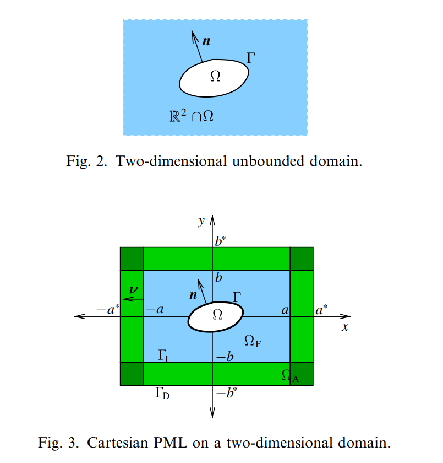
\includegraphics[width=7.437081857536404cm,height=7.770070838252656cm]{FDFD_tutorial-3.pdf}}

我们引入一些记号,记$\Omega_A$为吸收层,$\Gamma_1$为physical
domain与吸收层,$\Gamma_D$为吸收层与外部的交界面。我们需要两个吸收变量$\sigma_x,
\sigma_y$,分别关联垂直和水平的PML层,在转角处两个变量都作用。
\[ \left\{ \begin{array}{l}
     \Delta p_{\mathrm{F}} + k^2 p_{\mathrm{F}} = 0 \quad \text{in }
     \Omega_{\mathrm{F}},\\
     \frac{1}{\gamma_x}  \frac{\partial}{\partial x}  \left(
     \frac{1}{\gamma_x}  \frac{\partial p_{\mathrm{A}}}{\partial x} \right) +
     \frac{1}{\gamma_y}  \frac{\partial}{\partial y}  \left(
     \frac{1}{\gamma_y}  \frac{\partial p_{\mathrm{A}}}{\partial y} \right) +
     k^2 p_{\mathrm{A}} = 0 \quad \text{in } \Omega_{\mathrm{A}},\\
     \frac{\partial p_{\mathrm{F}}}{\partial \mathbf{n}} = g \quad \text{on }
     \Gamma,\\
     p_{\mathrm{F}} = p_{\mathrm{A}}  \quad \text{on } \Gamma_{\mathrm{I}},\\
     \frac{\partial p_{\mathrm{F}}}{\partial v_x} + \frac{\partial
     p_{\mathrm{F}}}{\partial v_y} = \frac{1}{\gamma_x}  \frac{\partial
     p_{\mathrm{A}}}{\partial v_x} + \frac{1}{\gamma_y}  \frac{\partial
     p_{\mathrm{A}}}{\partial v_y}  \quad \text{on } \Gamma_{\mathrm{I}},\\
     p_{\mathrm{A}} = 0 \quad \text{on } \Gamma_{\mathrm{D}},
   \end{array} \right. \]
where
\[ \gamma_x (x) = \left\{ \begin{array}{ll}
     1, & \text{if } |x| < a,\\
     1 + \frac{i}{\omega} \sigma_x (|x|), & \text{if } a \leqslant |x| <
     a^{\ast},
   \end{array} \right. \]
and
\[ \gamma_y (y) = \left\{ \begin{array}{ll}
     1, & \text{if } |y| < b,\\
     1 + \frac{i}{\omega} \sigma_y (|y|), & \text{if } b \leqslant |y| <
     b^{\ast}
   \end{array} \right. \]

\section{Finite difference frequency domain}

\

\end{CJK*}
\end{document}
